First looks great, puts the copy protection inside the app, a from of DRM\newline
communicate with server, authorize use of application\newline
does not prevent user from copying/transfering app, but copy useless since the app does run without the correct account\newline
google die ersten, andere folgen, anfangs problem, dass dadurch nur durch google store geschützt war, grund dafür dass evtl ein programmierer in meinen store kommt\newline

\subsection{Abstraction} \label{section:license-abstraction}
\begin{figure}[h]
    \centering
    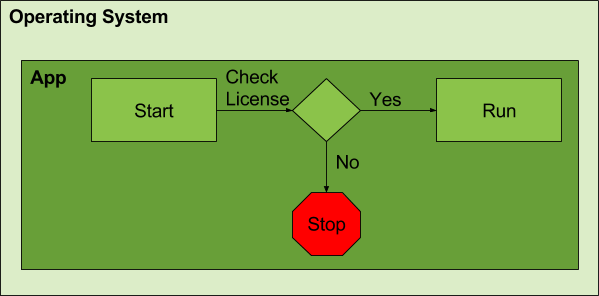
\includegraphics[width=0.8\textwidth]{data/verificationNow.png}
    \caption{Abstraction of the current license verification mechanism. The library is represented by (1)}
    \label{fig:verificationNow}
\end{figure}


basiert einzig auf der antwort vom server die ja oder nein ist


but there are problems as well
android's content protection are invalid when rooted
DRm can be bypassed
coupled with dex decompilkation big problem, app can be decompiled, modded and repackaged\cite{levinAndevcon}



Es muss generell immer abgewogen werden zwischen Reichweite und Sicherheit. Von Output den Lucky Patcher gibt, sind die auto patching modes für Google, Amazon und Samsung, die großen Player. Ein Developer muss seine App dort anbieten um Aufmerksamkeit zu bekommen. Deswegen sind diese Stores auch so gut "maintained" von Lucky Patcher.
Im Falle, dass ein Developer "Sicherheit" vorzieht und seine App in einem alternativen Store anbietet, gibt es zwei Scenarien. Entweder entwickelt jemand einen Custom Patch (dex oder native Angriff) wenn ein "allgemeines Interesse" besteht oder die App ist uninteressant und erhält keine Aufmerksamkeit, weder von LP noch Kunden.
